\section{Resultados}
\begin{frame}
	\frametitle{Control mediante Arduino Mega 2560}
	\begin{columns}
		\begin{column}{0.5\linewidth}
			\begin{figure}
				\centering
				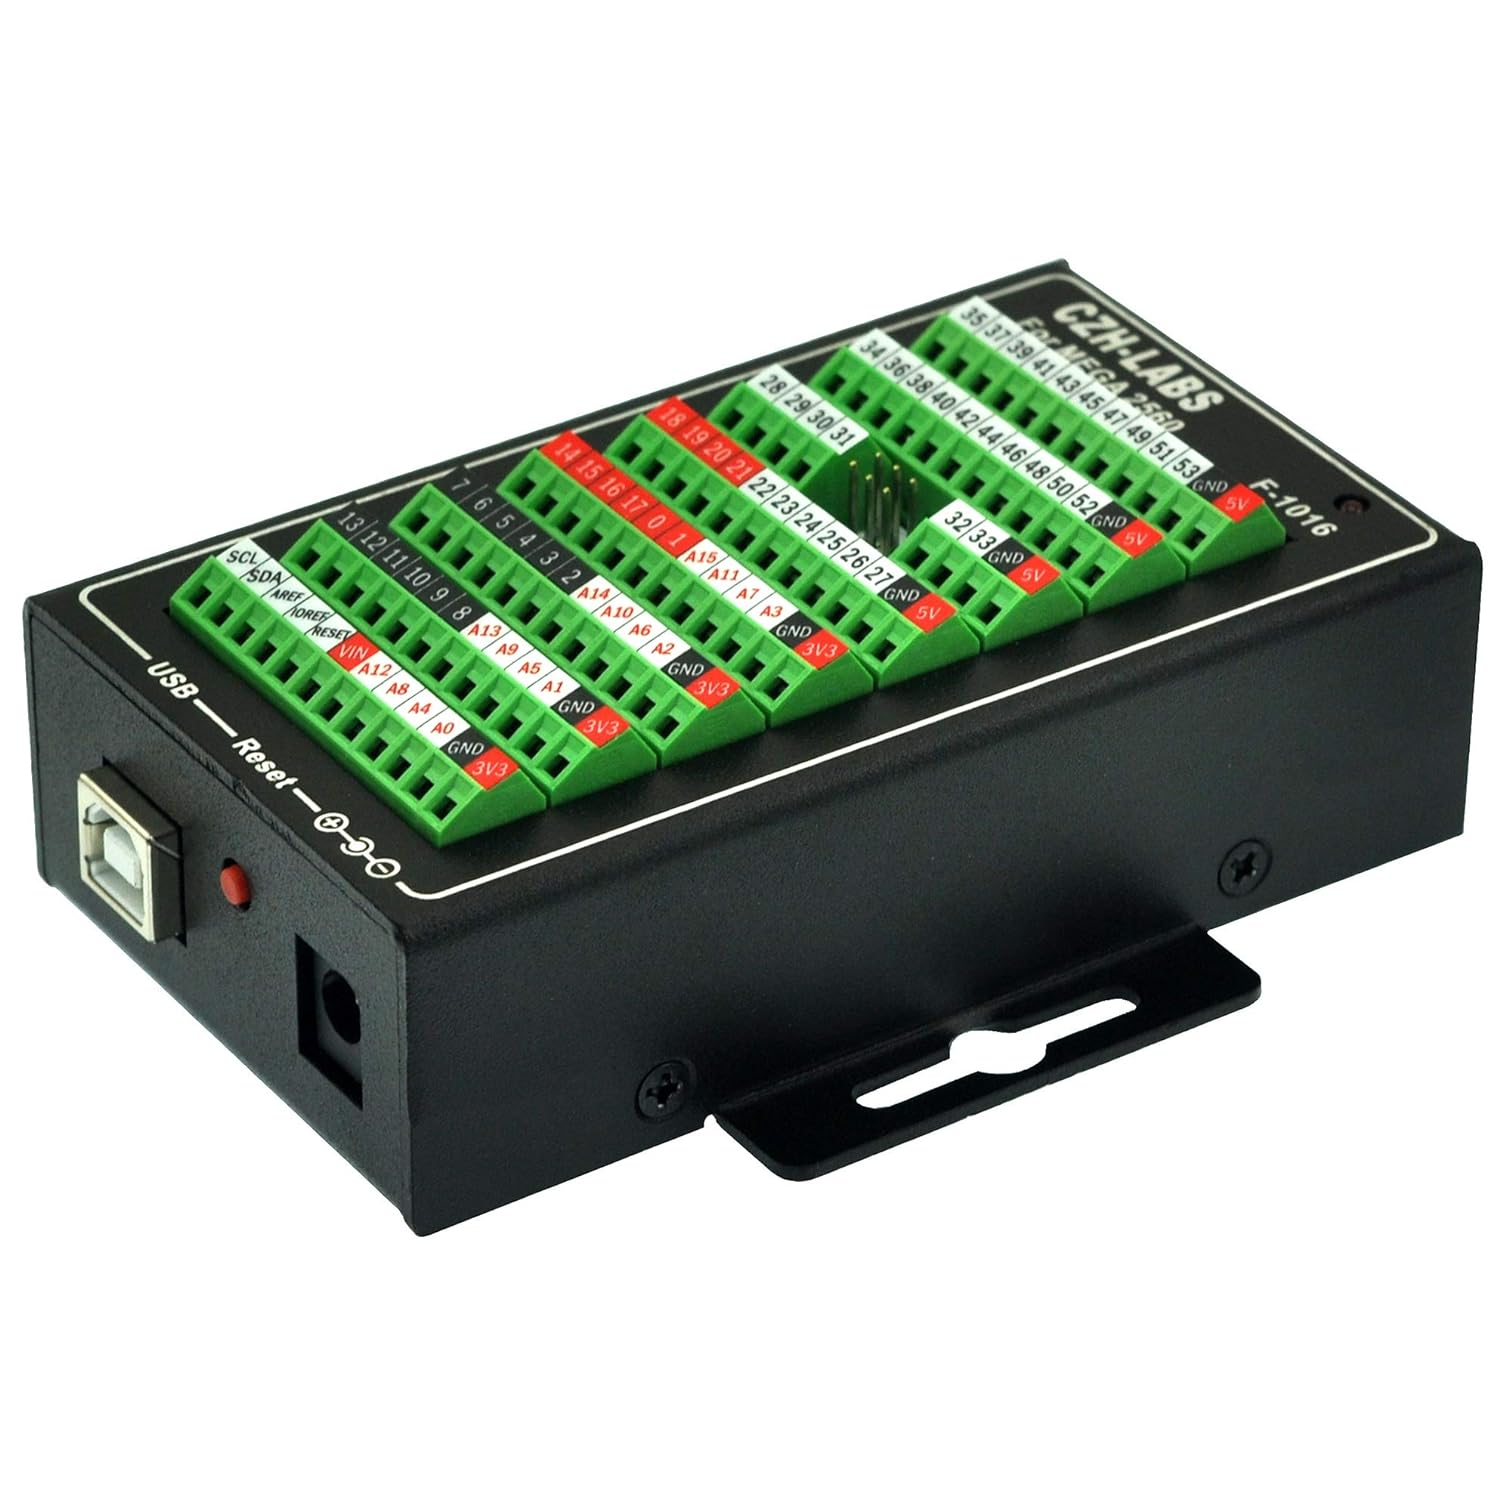
\includegraphics[
					height=60mm,
					width=\linewidth,
					keepaspectratio
				]{Resultados/Control/Arduino.png}
				\caption{Arduino con Shield}
			\end{figure}
		\end{column}
		\begin{column}{0.5\linewidth}
			\begin{figure}
				\centering
				
\includegraphics[
					height=60mm,
					width=\linewidth,
					keepaspectratio
				]{Resultados/Control/CPP.png}
				\caption{Programado en C++}
			\end{figure}
		\end{column}
	\end{columns}
		
\end{frame}

\begin{frame}
	\frametitle{Diagrama de clases del control}
	
	\begin{figure}
		\centering
		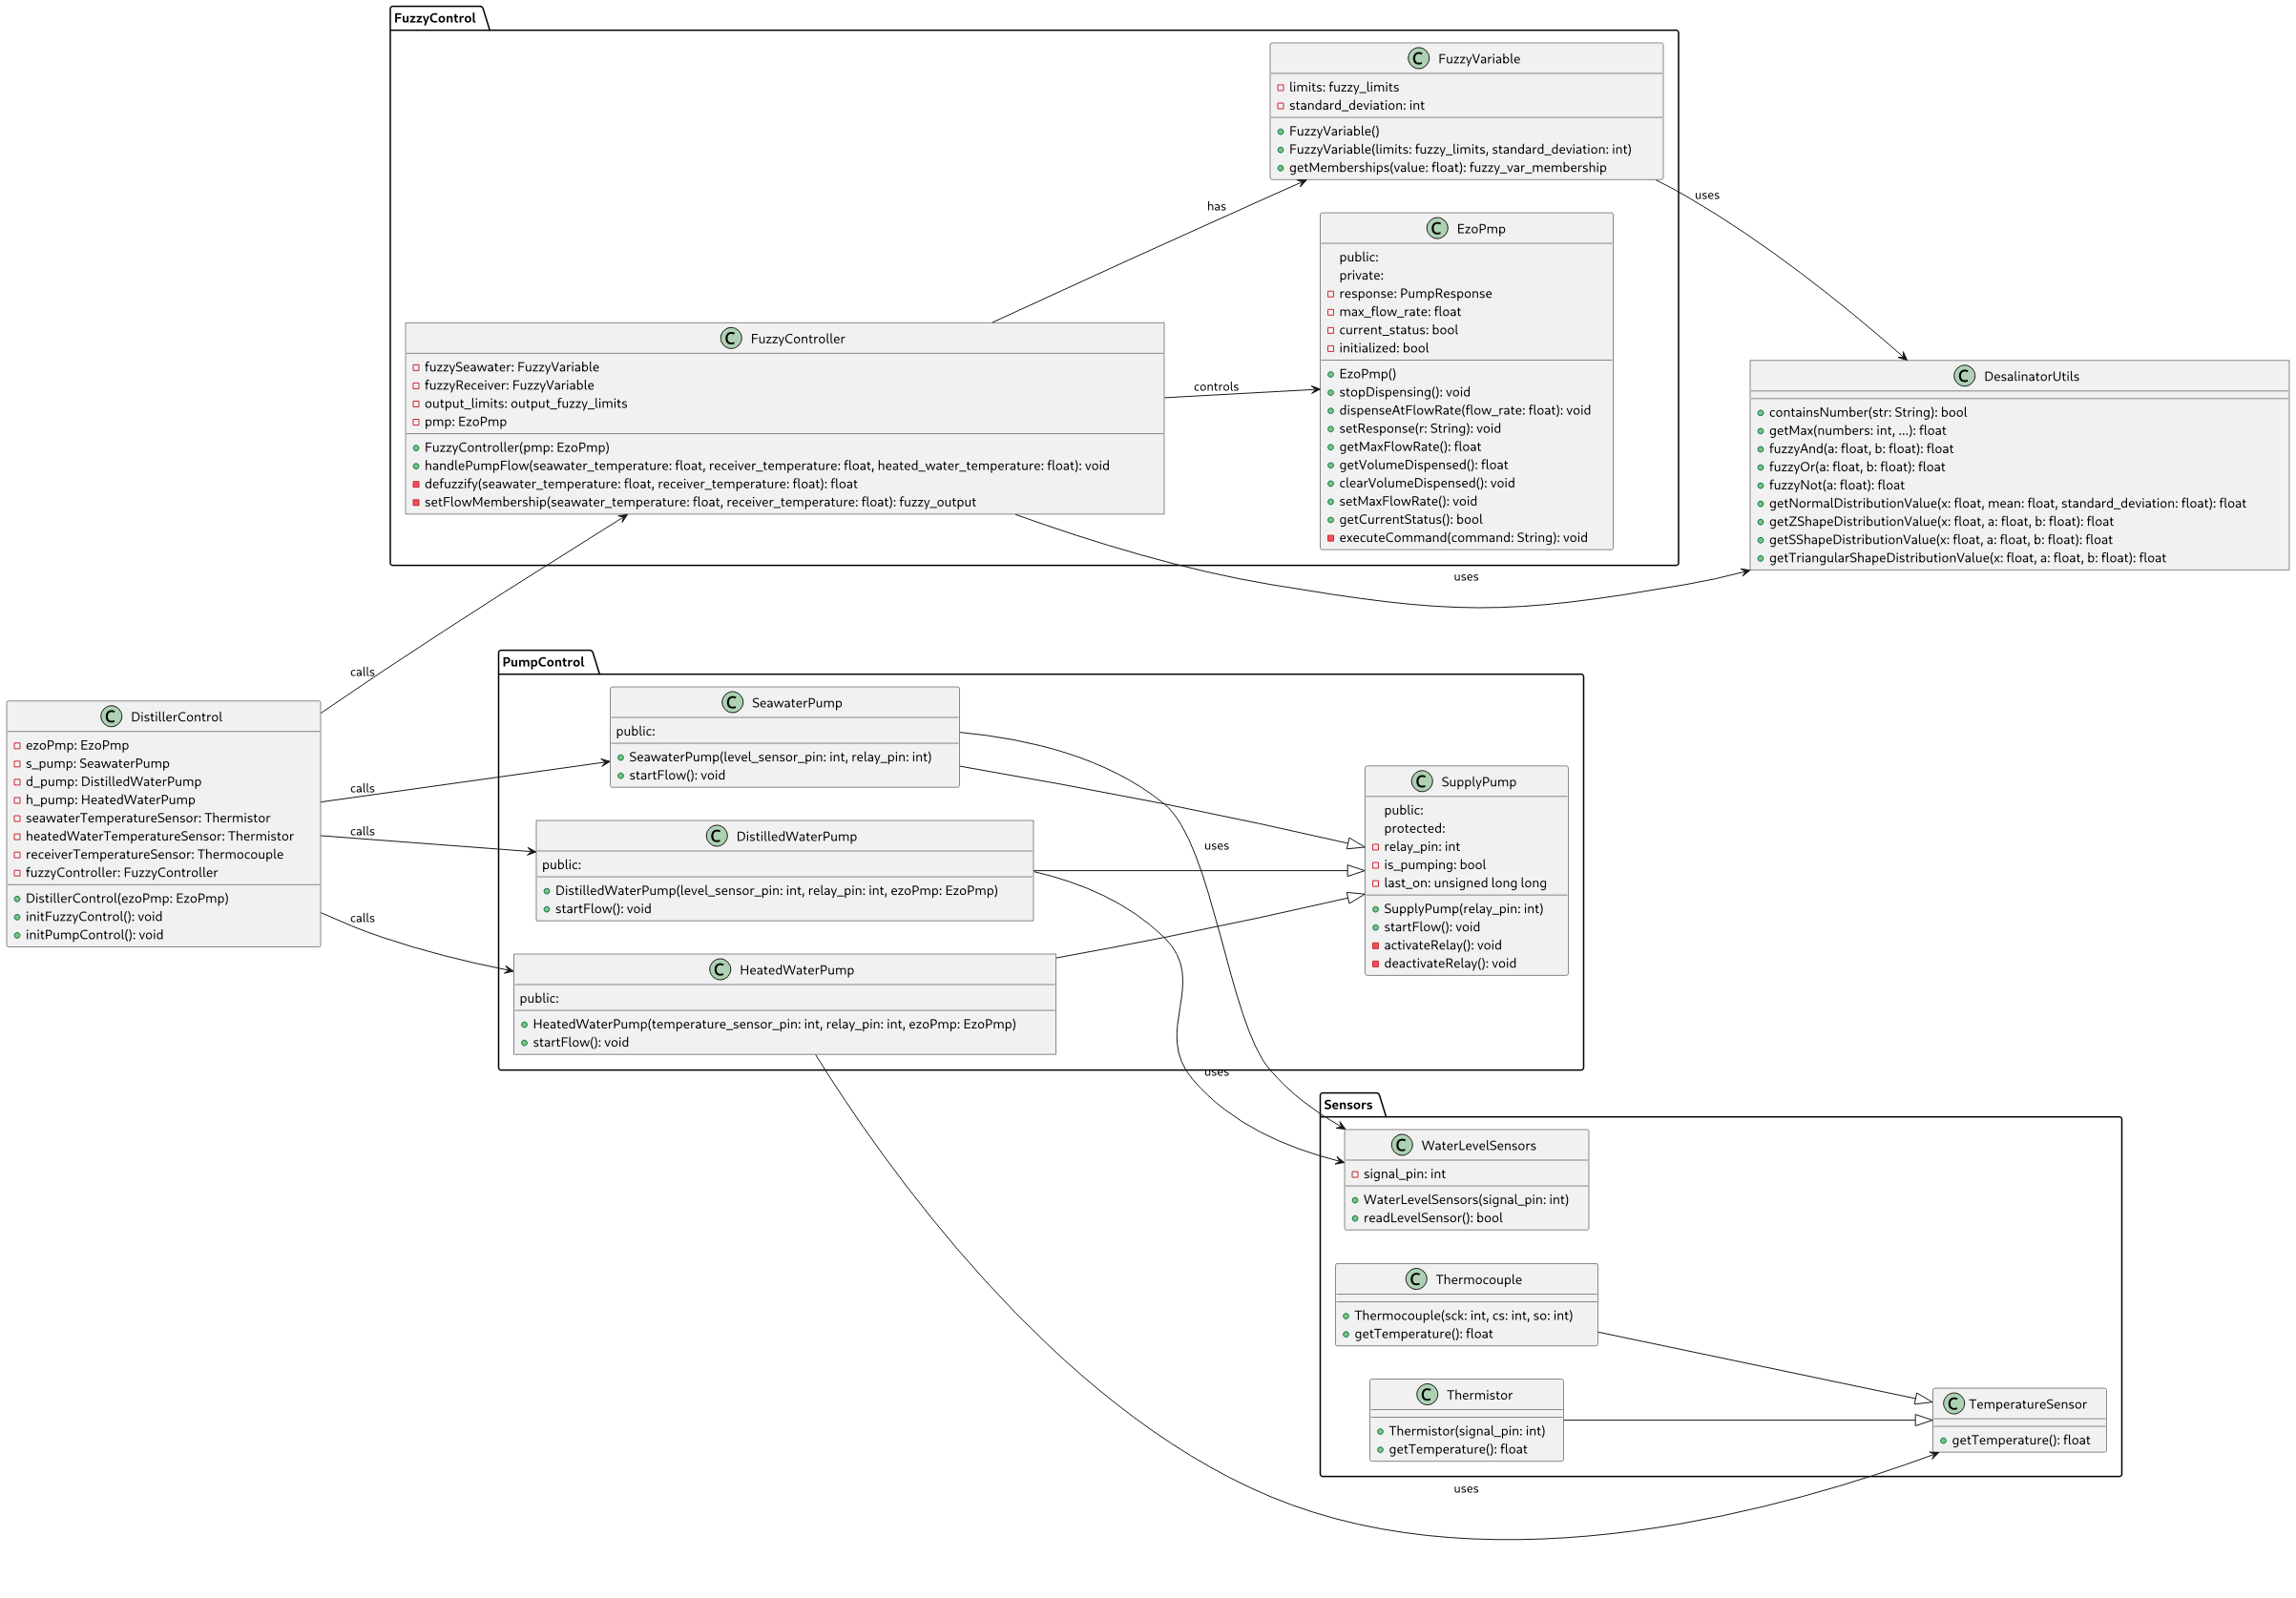
\includegraphics[
			height=\textheight,
			width=\linewidth,
			keepaspectratio
		]{Resultados/Control/ClassDiagram.png}
		\caption{Diagrama de clases del control}
	\end{figure}
\end{frame}

\begin{frame}
	\frametitle{Control del sistema}
	\begin{columns}
		\begin{column}{0.5\linewidth}
			\textbf{Control difuso}
		\end{column}
		\begin{column}{0.5\linewidth}
			\textbf{Control de los niveles de agua}
		\end{column}
	\end{columns}
	
	\begin{columns}
		\begin{column}{0.5\linewidth}
			Se encarga de regular el flujo de agua que fluye hacia el recibidor solar
		\end{column}
		\begin{column}{0.5\linewidth}
			Se encarga de llenar y vaciar los submódulos del módulo de reaprovechamiento térmico y bombeo. Usa sensores de nivel, tiempo transcurrido y temperatura del agua para tomar decisiones.
		\end{column}
	\end{columns}
		
\end{frame}